\def\mytitle{KIIIB}
\def\myauthor{Andreas M�ller s042809, David Emil Lemvigh s042809}
\def\affiliation{IMM@DTU}
%==================================================================================================
%   LUKES THESIS TEMPLATE 1.2
%   -------------------------
%   This template is based upon the offcial IMM PhD Thesis template, it is enhanced with a number 
%   of new features and a number of errors have fixed. This template is intended to be complied to 
%   PDF using PDFLATEX and is tested using the MiKTeX 2.9 LaTeX distribution. 
%   It is based on the official DTU-IMM Thesis template by Finn Kuno Christensen in 2009. 
%   -------------------------
%   Last Updated: 04-10-2011
%   Contact: lthhe@imm.dtu.dk
%==================================================================================================
%
%==================================================================================================
% DOCUMENT SETUP
%==================================================================================================
\documentclass[10pt,twoside]{book}                  %Official DTU-IMM Thesis document setup
%
%Set to 'print' for printed version, use 'net' for online version
\def\thesisversion{print} 			
%
%==================================================================================================
% PACKAGES
%==================================================================================================
\usepackage{LukeThesis}                             %Import Thesis base style 
\usepackage{listings}								% Import source listing package
\usepackage{color}
\usepackage[danish]{babel}

\usepackage{amsmath}
\usepackage{amssymb}
\usepackage{graphicx}				% Graphics
%\usepackage[ansinew]{inputenc} 		% UTF8 supprt
%\usepackage[T1]{fontenc}			% Some other characters

\usepackage{hyperref}				% So that \autoref works
\usepackage{url}					% So that \url works

\usepackage{tabulary}				% So we can have tables
\usepackage{booktabs}				% Better tables (aparently)

\usepackage[sort&compress]{natbib} 	% Better bibliography support
\bibpunct{(}{)}{;}{n}{}{,}			% Author-Year fix (apparently)

%\setlength{\parindent}{0pt}			% Sets paragraph indent to zero
%\setlength{\parskip}{7px}			% Adds space between paragraphs
%\setlength{\columnsep}{20px}		% Adds space between coloums

 


%input{PhDMacros}                                   %Thesis specific macros 
%
%==================================================================================================
% THESIS PROPERTIES (Modifiy these fields with your details)
%==================================================================================================
\def\thesisauthor{\myauthor}                     %Author
\def\thesistitle{\mytitle}		         		 %Title
\def\thesishandin{24-Febuary}					          %Submission date (Day-Month}
\def\thesisyear{2012} 							          %Submission year 
\def\thesisnumber{????}  						          %DTU-IMM Serial number (do not include year)
\def\thesisISSN{0000-0000}                          %ISSN number
\def\thesiskeywords{Keywords are, comma separated}  %PDF keywords 
\derivethesisprops                                  %Derive dependent properties

%==================================================================================================
% Source listing properties
%==================================================================================================
\definecolor{dkgreen}{rgb}{0,0.6,0}
\definecolor{gray}{rgb}{0.5,0.5,0.5}
\definecolor{mauve}{rgb}{0.58,0,0.82}

\lstset{ %
  language=Java,                % the language of the code
  basicstyle=\scriptsize,           % the size of the fonts that are used for the code
  numbers=left,                   % where to put the line-numbers
  numberstyle=\scriptsize,          % the size of the fonts that are used for the line-numbers
  stepnumber=1,                   % the step between two line-numbers. If it's 1, each line 
                                  % will be numbered
  numbersep=5pt,                  % how far the line-numbers are from the code
  backgroundcolor=\color{white},      % choose the background color. You must add \usepackage{color}
  showspaces=false,               % show spaces adding particular underscores
  showstringspaces=false,         % underline spaces within strings
  showtabs=false,                 % show tabs within strings adding particular underscores
  frame=single,                   % adds a frame around the code
  rulecolor=\color{black},        % if not set, the frame-color may be changed on line-breaks within not-black text (e.g. commens (green here))
  tabsize=2,                      % sets default tabsize to 2 spaces
  captionpos=b,                   % sets the caption-position to bottom
  breaklines=true,                % sets automatic line breaking
  breakatwhitespace=false,        % sets if automatic breaks should only happen at whitespace
  title=\lstname,                   % show the filename of files included with \lstinputlisting;
                                  % also try caption instead of title
  numberstyle=\tiny\color{gray},        % line number style
  keywordstyle=\color{blue},          % keyword style
  commentstyle=\color{dkgreen},       % comment style
  stringstyle=\color{mauve},         % string literal style
  escapeinside={\%*}{*)},            % if you want to add a comment within your code
  morekeywords={*,...}               % if you want to add more keywords to the set
}



%
%==================================================================================================
% SECTION NUMBERING SETUP
%==================================================================================================
\setcounter{tocdepth}{2}                            %2 adds sections up to subsections
\setcounter{secnumdepth}{3}                         %Subsubsections get a number when this is 3
%
%==================================================================================================
% THESIS STRUCTURE  (Modifiy to include more chapters etc)
%==================================================================================================
\begin{document}
%------------------------                                    
%Pre-frontmatter material
%------------------------
\prefrontmatter
%--------------------
%Frontmatter material
%--------------------
\frontmatter
\pagenumbering{roman}                               %Set frontmatter numbering style
\chapter{Summary (English)}

	The goal of the thesis is to explore the posebillities of a smart house system, with a minimal setup. The goal is to make it as easy as possible for the user, to install and use the system. The system should learn from the user's normal behavior, and eventually be able to copy the user's behavoir and take over control of the home, in a way that also reduces power consumption.
								             %English summary of Thesis
\markboth{}{}                                       %Set headings (left)(right)
\chapter{Summary (Danish)}
\begin{otherlanguage}{danish}

Målet for denne afhandling er at ...

\end{otherlanguage}								             %Danish summary of Thesis
\markboth{}{}                                       %Set headings (left)(right)
\chapter{Preface}

This thesis was prepared at the department of Informatics and Mathematical Modelling at the Technical University of Denmark in fulfilment of the
requirements for acquiring an M.Sc. in Informatics. 

The thesis deals with ... 

The thesis consists of ...
%==================================================================================================
% SIGNATURE AREA
%==================================================================================================
\vspace{20mm}
\begin{center}
	\hspace{20mm} Lyngby, \thesishandin-\thesisyear 
	\vspace{5mm}
	\newline
  %Update signature image file in line below
	
\includegraphics[scale=0.5]{figures/SignatureDummy.jpg}
\end{center}
\begin{flushright}
	\thesisauthor
\end{flushright}
% % % EOF % % %
								             %Preface
\markboth{}{}                                       %Set headings (left)(right)
\chapter{Acknowledgements}

	I would like to thank my....

					             %Acknowledgements
\markboth{}{}                                       %Set headings (left)(right)
%------------------
% Table of contents
%------------------
\newpage\mbox{}\newpage
\chaptermark{Contents}					
\renewcommand{\sectionmark}[1]{\markright{#1}}
\sectionmark{Contents}
\addtolength{\parskip}{-\baselineskip}
\tableofcontents
\addtolength{\parskip}{\baselineskip}
\renewcommand{\sectionmark}[1]{\markright{\thesection\ #1}}
%-------------
% Main content 
%-------------
\mainmatter


\chapter{Introduction}
\label{introduction}

In the recent years we have seen an increase in climate awareness. The subject is gaining more and more media coverage. A survey conducted from 2007 to 2008 by the international research organization Galllup\footnote{International research organization famous for making polls. http:/\slash ww.gallup.com}, shows that 82\% of americans and 88\% of europeans are very aware of the current climate issues we are facing such as global warming. In the same survey Gallup also concludes that 67\% of americans and 59\% europeans view global warming as a serious threat to them selves and their families~\citep[gallup--2009]{gallup-2009}. With the rise of concern with the general public, the demand for sustainable solutions increases.
According to the United States Energy Information Administration\footnote{http:/\slash www.eia.gov\slash }, the residential constituted 22\% of the total energy consumption in the US~\citep[eia--2011]{eia-2011}. 




\chapter{Analysis}
\label{analysis}




\section{Smart House Survey}
\label{smarthousesurvey}

\emph{``If I have seen further it is by standing on the shoulders of giants''} -- Isaac Newton

The beginning of any good project starts with a survey of what already exists in the field. 

Which smart house solutions already exist, and what are their capabilities? What are the industry standards, if any? This section will provide a representative selection of smart house solutions. However, it will not be an exhaustive survey of all smart house solutions.

First we will establish some basic classifications of smart houses, to better compare the different systems. All systems can contain switches, sensors and remote controls, the difference is the functionally they provide, and how they operate.

We distinguish between three types of systems, which are derived from the taxonomies presented in Boguslaw Pilich's Master Thesis ~\citep{Boguslaw} :


\subsection{Controllable houses}
\label{controllablehouses}

These are the simplest of the smart house solutions. Input devices like switches, remotes and sensors, can be setup to control output devices like appliance and dimmer switches, HVAC (Heating, Ventilation and Air Conditioning), etc. These solution may also include macros, e.g. where a single button may turn off all the lights in the home. 

\subsection{Programmable houses}
\label{programmablehouses}

These solutions incorporate some degree of logical operations, like having motions sensors not turn on the lights, if lux\footnote{A device for measuring the amount of light in a room. } sensors are above a threshold. They may be able to have scheduled task, e.g. turning down the thermostats during standard work-hours. The behavior of these systems have to be programmed by the manufacturer or the users. Consequently, changes in user needs require the system to be reprogrammed.

\subsection{Intelligent houses}
\label{intelligenthouses}

In these solutions some form of artificial intelligence is able to control the home. In computer science the term artificial intelligence is used very loosely. I our case we will define an intelligent house, as a system that is capable of machine learning. That means that the system is capable of evolving behavioral patterns based on empirical data~\citep{wikipedia-machine-learning}. Consequently, the system will over time adapt itself to changes in user needs.

The solutions presented, are some of the most widespread smart house solutions, and represents the three different types of systems: Controllable, Programmable and Intelligent houses.

$<$TODO hurtig conclusion om hver løsning, hvad synes vi om dem$>$

\textbf{INSTEON}

INSTEON is a controllable home control system, targeted at private homes. Nodes in the network can communicate using either RF signals or home's existing electrical wiring. A standard array of devices are supported: 

\begin{itemize}
\item Dimmers \& switches

\item HVAC

\item sprinklers

\item motion sensors

\item assorted bridge devices

\end{itemize}

INSTEON supports external application to be run on PC connected through a bridge devices to the network. By this logic it is technically possible to make the system programmable or even intelligent. However no commercial products providing these features currently exists. ~\citep{INSTEON}

INSTEON's solution is fairly widespread in the US, and is a successor to the Redoak X10 system, and is compatable with it's product.$<$does this matter?$>$ It represents what a commercial controllable smart house is capable of. It's functionaly very simplistic, but being able to communicate using the home electrical wiring, makes it a very non-intrusive system to install in an existing home. $<$lidt mere konklusion :)$>$



\textbf{Clipsal C-Bus}

Clipsal is targeted at large scale home control. The system is install in such prominent buildings as the Sydney Opera house, Wembly Stadium and many more. Nodes communicate over its own separate wired network, using the C-bus protocol. Each node has its own microprocessor, which allows for distributed intelligence. Each node can also be individually programmed, and communicate over the shared bus. This allows unconventional devices like motors for stadium roofs and many other devices to be part of the network. 

Clipsal's C-bus represents the flexibility and scalability programmable solutions on the market are able to achieve. It can also be installed in a private home. However, compared to other systems the rquirement of a separate wiring through-out a home can be a disadvantage. ~\citep{CBus} $<$skel mellem bus og system. diskuter distribuerede element mere$>$



\textbf{LK IHC}

LK IHC is targeted at private homes. It can be installed with a wired network, or using wireless communication. This solution tends to be build around simple wall switches, but with programmable scenarios, e.g. having a switch near the front door and the master bedroom that turns off all lights. It is a modular system, where modules like wireless communication or alarms, can be added to the base installation. 

The basic LK IHC installation is a controllable system. However, the modules can provide programmable functionality to the system, i.e. motion sensors normally control the lights, but if the alarm system is activated, the system can call 911. LK IHC was per 2008 installed in nearly 30\% of newly constructed building in denmark.~\citep{MSsurvey} ~\citep{LK IHC}. 

\textbf{MIT House\_n}

House\_n differs from the previous systems, as it isn't a finished implementation, but a framework for research projects. There aren't any widespread commercially available intelligent smart house solution on the market, or at least that satisfies our classification of intelligent. 

House\_n represent one of many smart environment, build by universities around the world. The smart environments are homes for one or more inhabitants, and are part of a living laboratory. The living lab part of House\_n is called PlaceLab, and is a one-bedroom condominium, inhabited by volunteers for varying lengths of time. These homes are designed for multi-disciplinary studies, of people and their pattens and interactions with new technology and smart home environments. Being university run smart homes, the work coming out of these facilities tends to be proof of concepts. ~\citep{MIT House_n}$<$diskuter house\_n som et ikke komplet produkt$>$

$<$TODO men fair nok, de er proof on concept, hvilke projekter findes der. Eller hvorfor snakker vi ikke om dem$>$

The projects shown in this survey represent the solutions currently available or in development. There are many different controllable and programmable solution commercially available, with INSTEON, Clipsal C-bus and LK IHC being some of the more widespread representative solutions. INSTEON being a simple controllable solution, Clipsal C-bus and LK IHK are both programmable smart house solutions, but where LK IHC is designed for private homes, the Clipsal C-bus system is better suited for larger buildings. 

MIT's House\_n in this survey represent that truly intelligent smart houses only exists in demonstration environments and as proofs of concept, and are not yet available on the commercial market.


One of the main problems with current home control solutions is that installing such a system is rather costly and requires installation and configuration, which is rarely trivial . Some of the more advanced systems on the market, such as the LK IHC, incorporate motion sensors and timers that automatically turn on and off lights or various appliances. These systems will save money over time, but they require extensive configuration or programming in order to function properly.
$<$mere konklusion, tilføj elementer til de enkelte huses konklusionser der kan refereres her$>$

\section{BIIIB}
\label{biiib}

Of all the qualities mentioned in our vision for the system, power saving is the most important. As seen in the survey above, this is an area where most modern home control systems falls short . Most systems are capable of providing only a modest reduction in power consumption, and some even increase the net consumption by adding the cost of running the control system. We want our system to differ from others on this specific aspect. In our system, reducing power consumption is the number one priority.

We want the users interactions with the system, to be as simple and familiar as possible. The user should only interact with the system through the wall mounted switches that are already present in all normal houses. 

We will accomplish this by creating a system that focuses on turning off all lights and appliances where they are not needed. There are several advantages to this approach, compared to attempting to reduce the power consumption of active appliances. The main advantage is that it provides the largest reduction in power consumption. Most people remember to turn off the light in the bathroom, when they leave it, but this is far less common for the kitchen, or dining room, and only the most environmentally conscious people would ever turn off the light in the living room when they got to the bathroom. This means that there is a lot of wasted energy in the normal household . 

Though we focus on controlling the lights in the house, the system must also be scalable so that in can incorporate other aspects, such as heating, ventilation, and electrical appliances. 

An other advantage is that it incorporates perfectly with all other power reducing technologies. Buying appliances that use less energy will still give you the same percentage of power reduction as in a normal house. 

This system will also eliminate the common problem of standby mode on many appliances such as TVs or stereos by having the appliance only in standby mode, when the user is likely to turn it on. The rest of the time the appliance is simply turned off.

Our approach to creating an intelligent house that is capable of predicting what the users want it to do, is to learn from what the user does and mimic these actions at the right times. To accomplice this, the system must do three things:

\begin{itemize}
\item The system must gather data on the users and their behavior in the house

\item The system must analyze the data in order to build a decision scheme on which it will base its actions

\item The system must be able control the house in real time, based on the decision scheme.

\end{itemize}

\section{Gathering data on the users}
\label{gatheringdataontheusers}

To mimic user actions, the system must first gather information on how the user interacts with the house. Therefore the first question we must answer is: What data should we collect on our users? In order for the system to effectively take over the users direct interactions with the house, we need to know two things. 

\begin{itemize}
\item What action needs to be done?

\item When shall the action be done?

\end{itemize}

The first question can be answered by monitoring the users direct interactions with the house. Since we have limited our system to handle lighting, this means monitoring the users interactions with the light switches.

The second question is a lot more complex. We need to collect data that can help us determine if the conditions are right for performing a specific action. We could of cause quite literally look at the time the action is performed, and then use that as a trigger, but this requires that users follow a very specific schedule.

To get a more detailed picture of when an action is done, we must analyze it relative to what the user is doing at the time. Since we're focussing on lighting this can be done simply by tracking the users movements. Thereby we will determine when an action shall be done based on where the user is, and where he is heading.

Perhaps the most obvious way of accomplishing this is by using cctv cameras. Using visual analysis is the most effective way of monitoring the user, as it will provide us with vast amounts of data on what the user is doing. By for example installing a fisheye camera in every room and use motion tracking on the video data stream, we can determine exactly where the user is, and what he is doing. While this is probably the solution that provides us with the most precise and detailed data, it does have one problem. Installing cameras in every room of the users house is, in out opinion, an unnecessary invasion of the users privacy. Even if the video data is not stored in the system, the presence of cameras will give many people the feeling of being watched in their own homes. 

An other approach would be to use a beacon worn by the user that sends out a digital signal. The system could then use multilateration\footnote{Multilateration is a navigation technique based on the measurement of the difference in distance to two or more stations at known locations that broadcast signals at known times

\chapter{Design}
\label{design}
} to pinpoint the exact location of the user. The beacon could be attached to the users keychain, incorporated into his cellphone, or, our personal science fiction favorite, injected under his skin. Like the camera approach this solution also has very high precision in tracking the user through the house. However,besides the point that the user might not always carry his keys or cellphone around, the main issue with this solution is scalability of users. Even though we limit the system to one user for now , we want a system that can be scaled to accommodate multiple users acting both and autonomously. Having to attach a beacon to every visitor coming into the house is gonna be an annoyance, and without it the house would not react to the visitor at all. 

The solution we chose is to use motion sensors. While this solution does not provide nearly the same precision in determining the users location as using fish eye cameras or multilateration, motion sensors does come with a range of other advantages. Motion sensor is a very cheap solution, compared to installing cctv cameras, and will be far less invasive on the user's privacy. The motion sensor solution will also work for any user in the house, and does not require the user to carry any beacon device like in the multilateration system. 

The system could easily be expanded by several other types of sensors as well. E.g. pressure sensors in the furniture, so the system can determine if there is someone present, even when motion sensors do not register them. There are several other examples of sensor technologies that could be incorporated in the system. Some will be discussed in the section `Future work'. 

For the moment we want to use as few hardware components as possible. There are two reasons for this:

\begin{itemize}
\item We want to keep the system as simple as possible from the consumers perspective. That means a system with as few components as possible.

\item Creating a system that analyses and mimics user behavior will have a lot of unknown variables that are hard to predict no matter how it is implemented. It will therefore be preferable to start out with a system that is stripped down to the bare necessaries and then add components as the need for them arises.

\end{itemize}

Because we want a system that is easy to install and configure, we have chosen not to inquire any information on the position of the motion sensors in the house.
This means that the system does not know where each sensor is located, nor which other sensors are in the same room as it. This does make analyzing the data a lot more complicated, but we want to stick with the idea of minimizing the installation and configuration. This way the installation process can be boiled down to putting up the sensors, plugging in the system, and pressing ``Start''. This also simplifies the maintenance of the system, when for example the user needs to replace a faulty sensor. This is again subscribes to the idea that the system should be smart, so the user does not have be.

Choosing to only monitor the light switches and using motion sensors to track the user greatly simplifies the data collection. Both the motion sensors and the switches generate events when they are triggered, and the system should simply store these events in a database. 

An alternative to this is to have the system analyze the data live, which would eliminate the need to store the event data. With this approach we do not have to store the events in the system, which over time could amount to a considerable amount of data. The problem is that if we should choose to modify the algorithms that analyze the data, we would effectively loose everything the system has learned so far. By storing the raw event data we can always recalculate a new decision scheme based on the collected data. This solution leaves us with a lot more options later on. The collection of data must still happen in real time. Since it is very important that the events are recorded exactly when they happen, the system must not stall in this process.

Since the project serves as a proof of concept for the idea of an intelligent house, we will need to collect real user data in order to properly evaluate our system. This is a necessary step in order to draw any meaningful conclusions on the system. There are two reasons for this:

\begin{itemize}
\item If we use generated data the house is not actually intelligent, it is merely acting on data created by the developers. The data we could supply the house would be based on how we think the user would behave. As developers it would be almost impossible not to be bias towards a behavioral pattern that is easy for the house to interpret, rather than how an actual user would interact with the house.

\item The project had a very large unknown element when we started out. No system quite like it have ever been created before, and it is almost impossible to predict how the system will react to different inputs. Though we are creatures of habit, our movement patterns do not run like clockworks. No matter how well we would generate training data using simulators, algorithms or any other artificial method, there would always be a doubt on how close to actual human behavior it actually is.

\end{itemize}

We do however not wish to create a fully functional physical installation, since this would take away too much focus developing the actual software system.

We chose to install a ``placebo'' system\footnote{A system where the sensors and switches have no actual effect on the house, but are merely there to collect data.} of wireless switches and sensors, to collect training data. This gives us the best quality training data for the system, without the expenses of installing operational wireless switches. With this training data, we can then use a simulator to evaluate that the system is learning properly. The data from the simulator is good enough to simulate simple movement patterns, to see which lights go on or off, as a simulated user moves from room to room. 

\section{Analyzing the collected data}
\label{analyzingthecollecteddata}

\emph{“If you torture data long enough, it will tell you what you want!”} -Ronald Coase 

Now that we have a lot of data on our users interactions with the house, we need to analyze the data in order for our systems AI to act on the collected data. To be more specific: We need to create a decision scheme that the AI can use as a base for its decision making. 

This is the critical part of the system. Collecting data, and acting based on an existing scheme are bot relatively simple tasks, however, designing the scheme to act, based on collected data, is far more complicated.

The purpose of analyzing the data is to find which specific situations that require the system to perform an action. Since the system does not know which sensors are located near which switches, the system will have to learn these relations based on the data collected. The simplest solution would be to have the system learn which switches and which sensors are located in the same room, and then create a ``link'' between them so the motion sensors control the light. This would result in what we have named the silvan[\^{}silvan] system. 

The silvan system is basically having a motion sensor turn on the light when triggered, and then have a timer turn off the light if the sensor is not triggered for a set amount of time. The main problem with this kind of system is that if the user does not trigger a motion sensor regularly, the light will turn off when the user is still in the room. This is commonly a problem in a room like the living room, where the user will likely spend an extended amount of time sitting still. This problem can be addressed by extending the light's timeout time. 

However, this brings us to the second problem. If the user is merely passing by a sensor, the light will still be turned on for its full duration. This greatly reduces the effectiveness of the system from a power saving point of view. 

A better solution is to attempt to identify the users behavior leading up to a switch event\footnote{An event generated in the system, by the user turning a switch on or off.
[\^{}silvan]: Danish building material retail-chain. }. Since the system only use motions sensors to track the users movements, these sensor events will form the basis for the data analysis. The system could simply look at what sensor was triggered right before a switch was activated, and the create a link between that sensor and the switch. This, however, would result in a system much like the silvan system described above. 

If we instead look at a series of sensor events leading up to a switch event, we will get a much more complex picture of what the user is doing. Since the switches in the house are located in fixed positions around the house, these movement patterns should repeat themselves relatively often. The movement patterns that lead up to a switch being turned off, will most likely also differ from a pattern leading up to a switch being turned on, since the user will be either entering or exiting a room. Once we have analyzed the data and identified the movement patterns related to a switch event, we need to create a decision scheme that the system can base its decision making on. That means we have to organize the analyzed data in a way so we easily can look up a specific pattern, and see whether it should trigger a switch action.

Unlike data collection, analyzing the data does not have strict time constraints. Since the decision scheme will be based on data collected over an extended period of time, the system will not benefit from having the decision scheme updated in real time. As a result the time constraints on analyzing the data will be quite loose, and should not pose as a restriction on the system. 

$<$the house should react to the user, and the user to the house$>$

\section{Controlling the house}
\label{controllingthehouse}

After we have collected and analyzed data the the final task is to have the system control the house in real time, using the decision scheme created from the analyzed data. The system must constantly monitor the user and attempt to match his movement pattern to those present in the decision scheme. As with data collection this has to happen in real time so the patterns are not corrupted.

\section{Requirement specification}
\label{requirementspecification}

Based of the analysis above we can now form a requirement specification for the project. The system shall collect data using motion sensors and by monitoring switches. This data should be stored as it is collected and without being manipulated.


In this chapter we will describe the design process, and discuss the major decisions we have made in regard to the system design. Since the system is research minded, and since the purpose of the project is to analyze the possibilities of developing an intelligent home control system using machine learning technology, we had to make some adjustments to the development process. The traditional waterfall model[\^{}waterfallmodel] for software development dictates that after finishing the project analysis, we would start designing how the system should handle the problems found in the analysis, along with the system architecture. Finally we would then implement the designed solution. With this project we were however faced with an additional challenge. When using machine learning you generally end up with a system that does not have an intuitive execution flow. This means that it can be almost impossible to predict the execution outcome because of the vast amounts of data that form basis for the systems decision making. This means that we have no way of verifying the validity of our proposed solution before implementing the system, or at least parts of it. Therefore we decided to approach the project by using incremental development instead[\^{}incremental-development]. 

In order to successfully apply this development model we must first divide the project into smaller parts, that can be implemented with each cycle. This design approach also inspired our final system design. Just like the development had several phases, where each phase had to be concluded in order to activate the next, the system will have similarly $<$huh?$>$ have different stages of operations. These stages are determined by the amount of data the system have collected on the user.

The system will have two different stages of operation. 

\begin{itemize}
\item In \textbf{The passive learning stage}, the system is running, but it has not yet collected enough data to make intelligent decisions. This stage is called the passive learning stage because the system is training it self by 

\item The system enters \textbf{the active learning stage} when there's enough data to attempt to manipulate the switches in the house. We call this the active learning stage, because the system now actively attempts to interact with the house's swithes . If the system makes a mistake and the user corrects it, e.g., the system turns off the lights and the user turns it back on, we can use that interaction to train our system further. In this case we can see it as the user punishing the system for making a mistake. The system will then adjust its decision scheme. This way the system will actively initiate a learning sequence. The system will remain in this stage indefinitely, and will continue to train it self using both passive and active learning. 

\end{itemize}

By using incremental development we are able to design and implement the system one stage at a time, and evaluate the passive part of the system before designing the active part.

In this chapter we will discuss the different stages of the system, the problems that are present in each stage, and the solutions designed to solve these problems. 

In the section ``Theory'' we will present the mathematical and statistical theory, that forms the basis for our machine learning algorithms.

This data collection in the system is very simple, and will not be discussed in this chapter. In the chapter ``Implementation'' this process will be described in detail.

The section ``The passive learning stage'' consists of three subsections. In the sections ``Event pattern'' and ``Decision table'' we will discuss how the system analyses the passively collected data. As discussed in the chapter ``Analysis'' using motion sensors can reduce the precision, and reliability of the collected data.In the subsection ``Zones'' we will discuss our approach to solve these problems. We will also provide a brief evaluation of the system in this stage, which will form the basis for the design of the active learning stage.

In the section ``The active learning stage'' we will discuss the additional processes that are present in this stage. These processes are made in response to the problems we have identified in the evaluation of the passive learning stage.

\section{Theory}
\label{theory}

\emph{``Stand back! Im going to try science!''} -Randal Munroe

In the core of our system lies a series of machine learning algorithms. In this section we will explain some of the basic concepts of machine learning, along with the statistical theory that it is based on.

\subsection{Machine learning}
\label{machinelearning}

The purpose of machine learning is to have the system evolve behaviors based on empirical data, rather than programming a specific behavioral pattern. By using the supplied data as examples of relationships between data events, the system can recognize complex patterns, and make intelligent decisions based on the data analyzed~\citep{ wiki-machinelearning}. 

With \textbf{supervised learning}[\^{}supervised-learning] the system is give labeled data consisting of examples of correct behavior. Because of both the human factor, and the imperfection of the motion sensors, the system will generate a certain amount of invalid data called noise. The algorithm will have to distinguish between what is proper training examples and what is noise.

In \textbf{Active learning}{\ldots} 

\subsection{Markov chains}
\label{markovchains}

A Markov chain is a mathematical system that under goes transitions from one stage to an other ~\citep{markov chains}. In a Markov system each step taken in a Markov chain is represented by a certain probability, based on the current state that the system is in. Formally:

\[P(X_{n+1} | X_n) \]

Here $X_{n+1}$ represents the next state, and $X_n$ represents the current state. And the entire notion is defined as the probability of the event $X_{n+1}$ given that event $X_n$ has just occurred. 

By arranging these values in a matrix you can create a lookup table for future reference.

\begin{table}[htbp]
\begin{minipage}{\linewidth}
\setlength{\tymax}{0.5\linewidth}
\centering
\small
\begin{tabulary}{\textwidth}{@{}lccccr@{}} \toprule
&$X_1$&$X_2$&$X_3$&$X_4$&$X_5$\\
\midrule
$X_1$&P($X_1| X_1)$&P($X_1| X_2)$&P($X_1| X_3)$&P($X_1| X_4)$&P($X_1| X_5)$\\
$X_2$&P($X_2| X_1)$&P($X_2| X_2)$&P($X_2| X_3)$&P($X_2| X_4)$&P($X_2| X_5)$\\
$X_3$&P($X_3| X_1)$&P($X_3| X_2)$&P($X_3| X_3)$&P($X_3| X_4)$&P($X_3| X_5)$\\
$X_4$&P($X_4| X_1)$&P($X_4| X_2)$&P($X_4| X_3)$&P($X_4| X_4)$&P($X_4| X_5)$\\
$X_5$&P($X_5| X_1)$&P($X_5| X_2)$&P($X_5| X_3)$&P($X_5| X_4)$&P($X_5| X_5)$\\

\bottomrule

\end{tabulary}
\end{minipage}
\end{table}


Each cell in the table represents the probability of entering the state represented by the cells row, assuming the system is currently in the state represented by the cells column.

\subsection{Markov chains with memory}
\label{markovchainswithmemory}

One of the most iconic features of Markov chains is the fact that they are memoryless. The probability of entering a new state is only based on the current state of the system. The states prior to the current have no effect on this probability. With ``Markov chains of order m'' the system has memory of the last m steps in the chain, and these affect the probability of entering future states.
This probability can be written as:
\[P(X_{n+1}|X_{n},X_{n-1}, ..., X_{n-m} )\]
Now the probabilities are calculated based on the pattern of steps made through the system rather than just the current state.

Since our probabilities are calculated based on collected data, we will not have to perform any complex statistical calculations.

\section{The passive learning stage}
\label{thepassivelearningstage}

When training the system, it will analyze the sensor data and look at all occurred event patterns. It will count the number of times each event pattern has been observed, as well as the number of times each event pattern has led to a switch being turned on or off respectively. Based on the number of times each event pattern has been observed, and has led to a switch event, the probability{\ldots} 

\subsection{Event patterns}
\label{eventpatterns}

$<$add reference to markov chains!!!!$>$ $<$ULTRA IMPORTANT ANDREAS!$>$


We want to be able to trigger the switches, based on more than just where the user is right now. We want to be able to look at where the user is coming from, and try to predict where the light needs to be turned on or off. So the light is already on when the user enters a room, and is turned off where it isn't needed. 

We want to determine the series of sensor events, or pattern, that leads up to a user turning the lights on or off, e.g. which sensors are triggered when a user goes from the couch to the restroom. If a series of sensor events, are less than some time interval apart, we consider them to be part of an event pattern. The time interval needs to be long enough, that a user moving around normally is seen as a continuous event pattern, and not broken into fragments. The time interval also needs to be short enough, that different user action, is seen as separate event patterns. For instance, a user going the kitchen to get a snack, and then returns to the living room, should ideally be seen as two separate event patterns.

With the idea of an event pattern, we can look at what patterns lead up to a switch event. And by extension of that analysis, when we observe an event pattern, we can determine the probability that it would lead to a switch event. 

\subsection{Decision Table}
\label{decisiontable}

In the core of the intelligent system lies the decision table. This is the product of the machine learning algorithm. The decision table is designed to be an efficient lookup table that the system can use as a decision scheme for its artificial intelligence. The decision table is designed as a Markov matrix, but we need the system to be able to handle Markov chains with memory, since we are tracking patterns, instead of single events. This effects the design of the Markov matrix.

Lets start by looking at the simple system with a pattern of length 2. Here we can simply use the Markov matrix described in the theory section. 

\begin{table}[htbp]
\begin{minipage}{\linewidth}
\setlength{\tymax}{0.5\linewidth}
\centering
\small
\begin{tabulary}{\textwidth}{@{}ccccc@{}} \toprule
switches $\backslash$ sensors&sensor 1&sensor 2&sensor 3\\
\midrule
switch 1&$P(switch 1 | sensor 1)$&$P(switch 1 | sensor 2)$&$P(switch 1 | sensor 3)$\\
switch 2&$P(switch 2 | sensor 1)$&$P(switch 2 | sensor 2)$&$P(switch 2 | sensor 3)$\\
switch 3&$P(switch 3 | sensor 1)$&$P(switch 3 | sensor 2)$&$P(switch 3 | sensor 3)$\\

\bottomrule

\end{tabulary}
\end{minipage}
\end{table}


For each set of sensor and switch events, the table above holds the probability of the switch event occurring, given that the sensor event has just occurred. This table acts as a relation table between the sensors and switches, in a system based on traditional Markov chains. In our system this means the pattern length is 1.

When we expand the Markov matrix to handle chains with memory, the matrix becomes more complicated. In the table above the number of cells is given by the number of sensors in the system multiplied by the number of switches in the system:
\[\#switches \cdot \#sensors\]
When we add a sensor event to the eventlist the number of cells in the matrix is multiplied by the number of switches again. This results in the general formula:

\[ \#switches  \cdot \#sensors^{pattern length} \]

As a result of this we see that for each event we add to the eventlist the matrix must be expanded by a new dimension. Thus a pattern length of n results in an n-dimensional matrix. 

As mentioned above we cannot at this moment determine what is the optimal pattern length, and therefore we must develop a system design that is flexible enough so that we can change the pattern length between each execution. This means that the decision table must be of n dimensions.


One advantage is that, since we are only interested in the users behavior related to his interaction with the wall switches, we only need to handle the patterns where the last event is a switch event. We must now go though our database, and for each switch event we must extract an eventlist consisting of that event and the n--1 sensor events preceding it. The decision matrix will consist of the number of times a pattern has occurred in the collected data. This value is then divided by the number of occurrences of the eventlist without the switch events. Thereby the value of each cell in the matrix will be classified as the number of times a pattern has been observed divide by the number of times the pattern excluding the switch event has been observed.


This value can also be interpreted as the probability that a specific switch event will occur after observing the pattern of sensor events. 

The system must also be able to handle patterns that are shorter than the maximum length, in case the pattern leading up to a switch event is smaller than the maximum pattern length. This could for example occur if the the interval between two events have been too long. As mentioned in the section above, the remaining places in the eventlist will then be filled with the value --1 preceding the existing values in the list.

The algorithm that handles the table generation looks as follows:

\begin{verbatim}
GenerateDecisionTable(events[]);
lastevent = 0
map decision_table
map denominator
que eventlist

for event in events
do
    if event = sensorevent
    do
        if event.time <= lastevent + pattern_interval
        do 
            push event to eventlist
            remove tail from eventlist
        else
            clear eventlist
        done
        insert event into denominator
        lastevent = event.time
    else
        if event.time <= lastevent + pattern_interval
        do
            insert event into decision_table
        else
            clear que
        done
    done
done

for entry in decision_table
do
    extract eventlist
    divide by matching denominator
done
\end{verbatim}


First the algorithm creates two maps: decision\_table and denominator. The decison\_table will, as the name suggests, hold the decision table. The denominator maps is used to keep track of the number of times each pattern of sensor events occur. This is used as the denominator when finding the probability in the decision table. The eventlist always contains the last n events in the system, unless the time between events exceeds the value stored in pattern\_interval. The algorithm now runs through the collected data in chronological order. 

If the current event is a sensor event, this is added to the eventlist, assuming that the time since the last event has occurred has not exceeded the pattern interval. The eventlist is now used to navigate through the n dimensional matrix denominator, and increase the occurrence of the pattern by 1.

If the current event is a switch event, this is added to decision table in the same fashion as with the denominator matrix. Since we are not interested in patterns that contains more than one switch even, the eventlist is now emptied.

Finally each value in the decision table is divided by the corresponding value in the deniminator matrix.

\subsection{Zones}
\label{zones}


In many cases to cover an entire room with sensors, the sensors end up overlapping in some areas. These overlaps can be used to increase the precision of the sensors. If two sensors triggers shortly after each other, then the user is in the zone where the two sensors overlap. In cases where multiple sensors triggers at the same time, it can be seen as one zone event.

Take (\autoref{zoneimg}) as an example, of three sensors which overlap a bit, and three paths past the sensors a, b and c. The paths b and c should only be observed as zone events by the system. While a path should look something like 1, zone 1 \& 2, 2, zone 2 \& 3, 3. depending on the cooldown of the sensors each event may be multiple times in the pattern.

\begin{figure}[htbp]
\centering
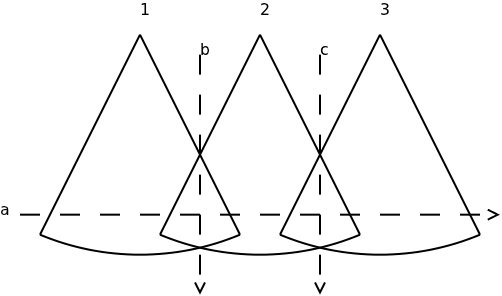
\includegraphics[keepaspectratio,width=\textwidth,height=0.75\textheight]{figures/zone.png}
\caption{Sensors with overlapping zones}
\label{zoneimg}
\end{figure}



Zones can also provide augment the system in other ways, than just increasing the precision of the motion sensors. When a user enters an area where sensors overlap, it might not be important which of them fires first. Without zone events, the path c would trigger either sensor 2 or 3 first, and these would be considered two distinct event patterns by the system. By looking at is as the same zone event no matter which sensor fired first, the system would be able to learn the intended behavior for path c faster by looking at is a zone event.

\section{The active learning stage}
\label{theactivelearningstage}

\subsection{Switch and sensor correlation}
\label{switchandsensorcorrelation}

It is beneficial to get a sense of which sensors are near which switches. And we have a lot of statistical data too look at. When a user turns a which on, it's most likely because there isn't light where the user intends to be in the immediate future. So it is possible to get an idea of which sensors are near a which, by looking at the interval shortly after a switch is turned on.

$<$TODO maybe talk about that is is less likely that a user will turn on a switch on, and then not enter that room$>$

When flicking a switch off, the user may be leaving the room, or just have entered the room to turn the switch off. Each of the two cases are just as likely as the other, but the sensor events in the interval leaving up to the off event is completely opposite. 

$<$TODO you could possebly look at the interval after it's turned off, and say there are less likely to be in the room, and then try to reduce the correlation for those sensors (NYI)$>$

Based on the statistical data it is possible to generate a table of probability that a sensor is triggered shortly after a switch is turned on, and by extension of that give a idea of which sensors are in the same room as a switch

\[ P(sensor_i | switch_j , \Delta t) = \frac{\sum 1_{sensor_i} (switch_i, \Delta t) }{\sum switch_j \ events } \]

The identity function $ 1_{sensor_i} (switch_i, \Delta t) $ is 1 if the sensor is triggered within $\Delta t$ after $switch_j$ is triggered, and is not therefor not counted twice, in the sensor triggeres multiple times after the same switch event.

So to reiterate $ P(sensor_i | switch_j , \Delta t) $ is the probability that $sensor_i)$ fires within $\Delta t$ after $switch_j$ fires.

\begin{table}[htbp]
\begin{minipage}{\linewidth}
\setlength{\tymax}{0.5\linewidth}
\centering
\small
\caption{Correlation table}
\label{ctable}
\begin{tabulary}{\textwidth}{@{}ccccc@{}} \toprule
&sensor 1 $(se_1)$&sensor 2 $(se_1)$&{\ldots}&sensor n $(se_n)$\\
\midrule
switch 1 ($sw_1)$&$P(se_1 | sw_1, \Delta t)$&$P(se_2 | sw_1, \Delta t)$&{\ldots}&$P(se_n | sw_1, \Delta t)$\\
switch 2 ($sw_2)$&$P(se_1 | sw_2, \Delta t)$&$P(se_2 | sw_2, \Delta t)$&{\ldots}&$P(se_n | sw_2, \Delta t)$\\
$\vdots$&$\vdots$&$\vdots$&$\ddots$&$\vdots$\\
switch m ($sw_m)$&$P(se_1 | sw_m, \Delta t)$&$P(se_2 | sw_m, \Delta t)$&{\ldots}&$P(se_n | sw_m, \Delta t)$\\

\bottomrule

\end{tabulary}
\end{minipage}
\end{table}


\subsection{Correlation based timeout}
\label{correlationbasedtimeout}

Ideally the system will turn off the light by detecting off patterns, but in the learning stage or if the user changes behavior, this isn't reliable. We want to avoid is the light being on longer than it needs to, even if the system doesn't detect the off pattern. The user leaves a room and doesn't realize the light is still on, or expect the system to turn off the light on it's own, causing a necessary waste of energy.

We wanted to make a situation where no matter what happens the light is eventually turned off. The system has a timer for each switch, and as the user is detected by the sensors, the timer is extended based on the correlation to the switch. In a real scenario it's very like for any sensor to have at least some correlation to any switch, however low it might be. So the system has to avoid having all sensors extending the timeout ever so slightly, essentially keeping the light on for as long as sensors events keep firing somewhere. Therefor the correlation has to be above some threshold in order to extend the timeout. Ideally only sensors in the same room as the switch are extending the timeout.

\subsection{Timeout adjustment}
\label{timeoutadjustment}

The problem with a timeout based solution, is people sitting still. Most people have experience controllable or programmable smarthouse solutions, where motion sensors keep the light on for some amount of time. And it tend to work great in spaces where people are passing through, hallways, carports, et cetera. But in places where people some times sit still, be it working or relaxing, motion sensors won't be triggered, and user end up having to get up or wave their arms to keep the lights on. So we allow the system to keep the light on for longer duration in some areas, based on which sensors are triggered, and also a way for the system to learn where these areas are. As already stated the base timeout is based on the correlation, which means sensors close to the switch will keep the light on longer. A common scenario in a home would be a user laying on a couch watching TV. So we want the system to be able to keep the lights on longer, if it detects that the user is on the couch. If a timer runs out, the system turns the switch off, and if the user immediately turns it back on again, the system takes that as a punishment for it's behavior. The system reacts by increasing the timeout those sensors have to the switch. Adversely if a timer runs out, and the user doesn't take any action, it assumes it's behavior was correct, and decreases the timeout.

\subsection{Confidence}
\label{confidence}

A key transition of the system, is when does it go from the untrained stage to the learning stage? When is the system confident enough to take over control of the home. In the ``placebo'' setup, the system couldn't enter the learning stage, since it couldn't control the lights. Therefor this functionality wasn't implemented, but is still key feature of the system, and should be discussed in this report. 

There are two main metrics we believe should determine when the system is confident enough:
The system should start attempting to control the home, once it is confident enough, to act upon the decision schemes it has learned. But the system needs to have some quantifiable metric to determine it's confidence, before it start to take over control of the home:

\begin{enumerate}
\item The probability in the decision scheme must be above some threshold. $P(switch_i | pattern_j) > \varphi $

\item The specific $pattern_j$ must have occurred at least some number of times.

\end{enumerate}

Exactly what the threshold should be, is up to speculation and could be determined through experimentation, once the system in ready to enter the learning stage. The second rule is to make sure, the system doesn't start acting based on patterns only observed once.

\chapter{Implementation}
\label{implementation}

\begin{itemize}
\item Description of the system components

\item The implementation section should allow a skilled programmer to maintain the software

\item \textbf{Remember, the most important documentation of the implementation is comments in the code!}

\end{itemize}

\section{The physical setup}
\label{thephysicalsetup}

\begin{verbatim}
<more information on z-wave>
\end{verbatim}





In order to collect training data, we installed wireless switches and PIR sensors\footnote{Passive infrared sensors.} in a home (\autoref{hellebaekgade}). The placebo switches were placed next to the normal switches controlling the light for each room, in all cases being the switch closest to the entrance. We installed a total of 10 motion sensors and 5 switches throughout the apartment, that collected data non stop for a period of two weeks.

Each room have one or more PIR sensors, averaging 2 per room, with one lest in the restroom and an additional sensor in the living room. When placing the sensors, the system can obviously only learn from behavior in areas covered by sensors. So sensors should provide as close to full coverage as possible, with special emphasis on making sure the entrances are covered. 

\begin{figure}[htbp]
\centering
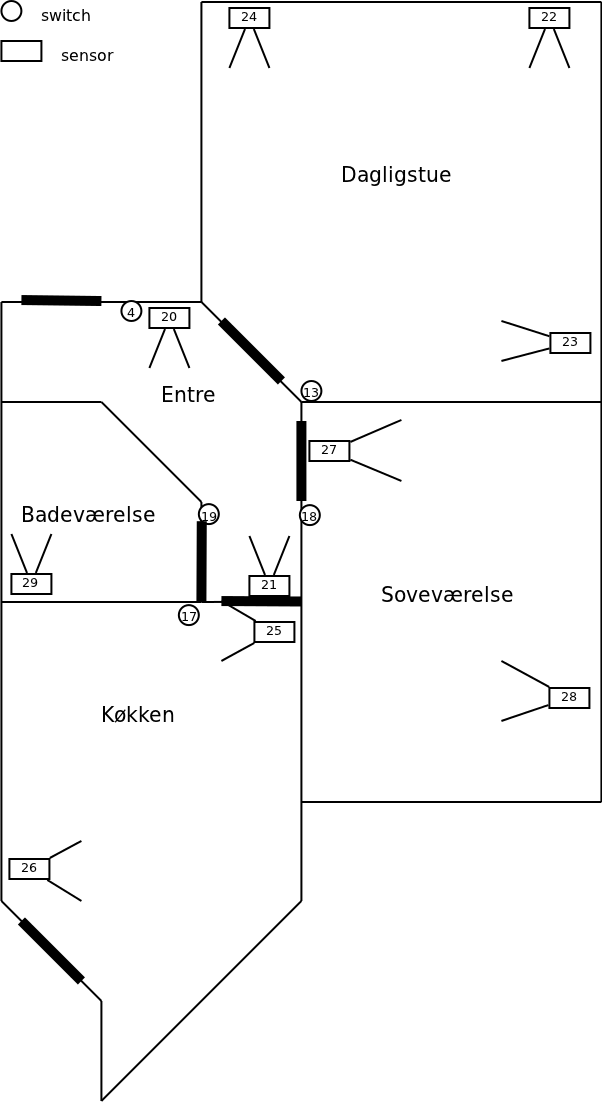
\includegraphics[keepaspectratio,width=\textwidth,height=0.75\textheight]{figures/hellebaekgade3.png}
\caption{Map of the testing environment with sensor and switch locations}
\label{hellebaekgade}
\end{figure}



The wireless nodes we have available communicate using the Zensys Z-Wave protocol. We setup a mini PC with a Z-Wave serial device, and configured all PIR sensor and switches to send notifications to the PC, when they where activated. The PC ran a Z-Wave API, which we added a listener to, so that sensor and switch event was logged to a SQL database.

\begin{table}[htbp]
\begin{minipage}{\linewidth}
\setlength{\tymax}{0.5\linewidth}
\centering
\small
\caption{Database table for sensor events}
\label{sensortable}
\begin{tabulary}{\textwidth}{@{}ll@{}} \toprule
\multicolumn{2}{c}{sensor\_events}\\
\midrule
id&Integer\\
timestamp&Timestamp\\

\bottomrule

\end{tabulary}
\end{minipage}
\end{table}


\begin{table}[htbp]
\begin{minipage}{\linewidth}
\setlength{\tymax}{0.5\linewidth}
\centering
\small
\caption{Database table for switch events}
\label{sensortable}
\begin{tabulary}{\textwidth}{@{}ll@{}} \toprule
\multicolumn{2}{c}{switch\_events}\\
\midrule
id&Integer\\
timestamp&Timestamp\\
status&Boolean\\

\bottomrule

\end{tabulary}
\end{minipage}
\end{table}


\section{Simulator \slash  AI interface}
\label{simulatoraiinterface}

We have a smart house simulator available, which will be extended with an AI module, implementing the features discussed in this report. The simulator is implemented in scala, so an obvious choise would be to implement the AI in scala aswell. However work with the simulator in the initial stages of the project, showed that our programming speed in scala was too slow to get any meaningful amount of work done. The scala language is build upon Java, and both languages compiles to bytecode in \emph{.class} files. A result of that is that Scala and Java interface very easily, and Scala code can invoke Java methods and vice versa. We chose to implement the AI in Java, working in a language we're well-versed in, to increase our productivity and quality of the code.


\section{Configuration}
\label{configuration}



\section{Decision Matrix}
\label{decisionmatrix}

Antallet af gange den klasse har skiftet navn{\ldots} I've lost count{\ldots}
 - svaret er 4
$<$TODO Andy, you deal with it$>$

\section{Event patterns}
\label{eventpatterns}

To make lookups based on the lastest event pattern, each new sensor event needs to be a matched to see if it's part of a pattern.
As each sensor and switch event is received by the system, a list of the most recent event pattern is maintained in an EventList. 

EventList determines if the lastest event is part of the pattern, and determines if a zone event has occured (if set to use zone events). 

The invariant of the EventList, is that after an event is added, the event list contains the current event patttern. This pattern can then be used to determine if any switches should be turned on or off.

\section{Correlation table}
\label{correlationtable}



\subsection{Correlation statistical generation}
\label{correlationstatisticalgeneration}

Correlation calculates the probability that a sensor is correlated a switch. It scans the database, and looks at the interval just after a switch is triggered. The sensors that triggered in the interval, are counted for that interval, in a way thay they're only counted once per switch event. If a multiple switch event are triggered in the same interval, the sensor events in the overlapping intervals should be counted for each of those switches. Having the number of times each switch is triggered, and each sensors triggeres with the given time interval, it's then calculated the probability that $ sensor_i $ is triggered, given that a $ switch_j $ was turned on atmost $ \Delta t $ ago. This gives the statistical correlation probability table. 

To this the correlation confirmations in the database, is then added. Each row in the database table contains the accululated correlation correction for that switch \slash  sensor pair. The correlation correction is simply added to the correlation based on the statistical data.

The resulting correlation table is allowed to have probabilities above 100\%, which is inteded as destribed in 

\subsection{Correlation correction}
\label{correlationcorrection}

When a switch is turned on, a timer is started for that switch. If a correlated sensor is triggered, it timer is extended. The duration is determined by the correlation between the sensor and the switch, higher correlation gives longer timeouts. If the switch is turned off, the timer is stopped. If the timer runsout a timeoutevent is triggered, and the light is turned off, and a new timer is started, to verify that no manual overrides occur. If the a manual override occurs (e.g. the user turns the switch on again, while the timer is running), the system is ``punished''. The system increases the timeout time, by increasing the correlation between the switch and the first sensor triggered after the switch was turned off. If no manual override occurs, the system was correct in turning off the light, and lowers the timeout time, by reducing the correlation between switch and the last seen sensor before the switch was turned off.

These correlation corrections are stored in a separate table in the database. The correlation use for the timeout is based on both the statistical correlation, and these correlation corrections. The correlation corrections increase or reduce the correlation by 10 percent points. The system allows correlations higher than 100\%, this gives the intended behavior that a switch may have a longer timeout than what is default.

\begin{table}[htbp]
\begin{minipage}{\linewidth}
\setlength{\tymax}{0.5\linewidth}
\centering
\small
\caption{Database table for correlation corrections}
\label{corrcorrtable}
\begin{tabulary}{\textwidth}{@{}ll@{}} \toprule
\multicolumn{2}{c}{correlation\_confirmation}\\
\midrule
switch&Integer\\
sensor&Integer\\
correlation&Float\\

\bottomrule

\end{tabulary}
\end{minipage}
\end{table}


\section{Timers and timeout}
\label{timersandtimeout}

Timers are implemented in the Timer and Sleeper class. Sleeper is a fairly simple class, it sleeps starts a new thread, sleeps for a given time, then fires a timeout event to a given timeout listener. Timer simply holds a map, where each switch can set a timeout. Timer creates a sleeper object, and puts in the map. The sleepers can then easily be monitored and interrupted if needed. 

To received the timeout events the SmartHouse class implements TimeoutListener. 

\chapter{Evaluation}
\label{evaluation}

\emph{``If it compiles, it is good; if it boots up, it is perfect.''} -- Linus Torvalds

\begin{itemize}
\item Evaluation should document that the goals have been achieved

\begin{itemize}
\item Functional requirements (i.e., testing)

\item Non-functional requirements (e.g., performance)

\end{itemize}

\item Definition of the evaluation strategy

\begin{itemize}
\item Qualitative-\slash quantitative evaluation

\item Software testing

\begin{itemize}
\item white-box\slash black-box

\item testing levels
*unit testing, integrationg testing, system testing, acceptance testing

\end{itemize}

\end{itemize}

\item summarised output from the evaluation
*output should be explained

\begin{itemize}
\item provisional conclusions should be presented

\end{itemize}

\end{itemize}

\begin{figure}[htbp]
\centering
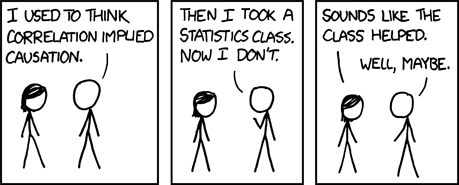
\includegraphics[keepaspectratio,width=\textwidth,height=0.75\textheight]{figures/correlation.png}
\caption{XKCD Correlation}
\label{correlation}
\end{figure}



\section{Software testing}
\label{softwaretesting}

For the relative simple and predictable module EventList, we have done some white-box testing, using JUnit tests. Making sure it correctly detect zones,that pattern ordering is preserved, and old event are purged when new events are added according to the pattern length and interval parameters. The more complex modules DecisionMatrix and Correlation are tested and evaluated based on the gathered user data.

\section{Decision matrix}
\label{decisionmatrix}

A bit of sensor meta data:

45.628 sensor events
346 switch events, 194 on and 152 off. The observant reader might wonder why there are a lot more off commands than on commands? The short answer is the user's may have forgotten to press the placebo switches from time to time.

$<$TODO 111 also being the theoretical maximum of unique patterns, for a home with 10 sensors
1 : no sensors, just switch
10 : single sensor events then switch event
100 (10*10) : two sensor events then switch event
I'm slightly impressed$>$

\begin{table}[htbp]
\begin{minipage}{\linewidth}
\setlength{\tymax}{0.5\linewidth}
\centering
\small
\caption{Statistics about the Decision matrix}
\label{dtablemetadata}
\begin{tabulary}{\textwidth}{@{}ccccc@{}} \toprule
\multicolumn{2}{c}{Settings}&\multicolumn{3}{c}{Unique observed patterns}\\
Pattern length&Zones enabled&Movement patterns&On patterns&Off patterns\\
\midrule
2&No&111&89&72\\
2&Yes&928&147&120\\
3&No&910&142&117\\
3&Yes&4097&225&171\\

\bottomrule

\end{tabulary}
\end{minipage}
\end{table}


With zones enabled, the system looks at the event patterns both with and without zone. Which is why there are more observed on patterns, than actual on commands, when the pattern length is longer than three and zone detection is on. 



\section{Correlation}
\label{correlation}

In this section we are going to evaluate how well correlation, based on the generated user data, matches to the actual setup. Is the system able to get accurate estimates of which sensors and switches are in the same room. We are also going to evaluate how well the correlation based timeout would work, with or without correlation corrections. Prior to looking at the actual data, we want to state some resoanable goals we want the system to achieve for the correlation probabilities:

\begin{enumerate}
\item A sensor should have the highest correlation to the switch in the room it is in.

\item Some correlation threshold should exist, so that sensors and switches in the same room are above the threshold, and those not in the same room are below the threshold.

\end{enumerate}

\begin{table}[htbp]
\begin{minipage}{\linewidth}
\setlength{\tymax}{0.5\linewidth}
\centering
\small
\caption{Correlation table, based on statistical data. $>$ 40\% in bold, 40--20\% in italic.}
\label{ctabledata}
\begin{tabulary}{\textwidth}{@{}rlcccccccccc@{}} \toprule
\multicolumn{2}{c}{Switches}&\multicolumn{10}{c}{Sensors}\\
&&20&21&22&23&24&25&26&27&28&29\\
\multicolumn{2}{c}{}&\multicolumn{2}{c}{Hallway}&\multicolumn{3}{c}{Living room}&\multicolumn{2}{c}{Kitchen}&\multicolumn{2}{c}{Bedroom}&WC\\
\midrule
4&Hallway&\textbf{0.4}&\textbf{0.67}&0&0.2&0.13&0.07&0&0&0.07&0\\
13&Living room&\emph{0.35}&\emph{0.23}&0.12&\emph{0.27}&\textbf{0.42}&0.04&0.04&0.08&0.08&0\\
17&Kitchen&\emph{0.22}&\emph{0.28}&0&0.03&0.17&\emph{0.39}&\textbf{0.58}&0.14&0.03&0.03\\
18&Bedroom&0.1&0.13&0&0&0.03&0.03&0&\textbf{0.57}&\textbf{0.6}&0.03\\
19&WC&\emph{0.29}&\emph{0.29}&0.06&0.09&0.08&0.06&0&0.07&0.03&\textbf{0.75}\\

\bottomrule

\end{tabulary}
\end{minipage}
\end{table}


The correlation table (\autoref{ctabledata}) is based on collected data from the testing environment. The first criteria holds, that all sensors have the highest correlation with the switch in the room they are in.
The send criteria does not hold for all correlations. Most correlation probability for sensors and switches in the same room are above 40\%. All correlations for switches and sensors not in the same room are below 40\%. But three sensors have correlations lower than 40\% to the switch in the room they are in, and one of them as low as 12\%. In the living room, two sensors not only have correlations below 40\%, but correlations below those of sensors in the adjecent hallway. 

As can be seen in the overview of the appartment (\autoref{hellebaekgade}), the sensors 22 and 25 are located in the far end of the rooms from the switch and doorway. Since the calculated correlation probabilities are based on the time interval just after the light is turned on, it makes sense that these sensor, being relatively far away from the switches ends up with a lower correlation. 

Sensor 23 is positioned to monitor the sofa in front of the TV, and the data suggest that it only detect the user if he go to the sofa immediately after he enters the room. So not all sensors neccesarily trigger in a room, depending on what the user decides to do in the room. 

So in this case, the correlation still gives an excelent estimate of which switches and sensors are in the same room, by looking switch each sensor has the highest correlation probability too. 

One thing to note is, these are the probabilities based solely on the statistical data, and that correlation corretions would be added onto this schema. So it is not a perfect reflect of which sensors are in the same room each switch, on it is own. But it does gives a good approximation.

\subsection{Correlation based timeout}
\label{correlationbasedtimeout}

The implemented functionality of the correlation table, is to determine the timeout when a switch is turned on. So how well is the correlation table able to keep the light on where it's needed? Different areas should have different timeouts, but the most important for the system is to have long timeouts in areas where the user is likely to be still for extended periods of time, while still wanting the light to remain on. The most obvious area would be the sofa, 

\chapter{Conclusion}
\label{conclusion}

\begin{itemize}
\item summarises all the result of the project

\begin{itemize}
\item what was the problem?

\item what has been achieved?

\end{itemize}

\item presents final conclusions
*summary of provisional conclusions

\begin{itemize}
\item further conclusions drawn from the sum of evidence

\end{itemize}

\item presents directions for future work

\begin{itemize}
\item new problems identified through the project

\item outline the possible evolution curve of the software

\end{itemize}

\end{itemize}

\section{writing good conclusions}
\label{writinggoodconclusions}

\begin{itemize}
\item What was the problem?

\begin{itemize}
\item Remind the reader of the context and project goals

\end{itemize}

\item What was the proposed solution?
-Remind the reader of the proposed solution
 -what was done in the project

\item How did we evaluate the proposed solution?
-Summarize results of indicidual experiments.
 -this inclydes any testing of software in development projects
-Draw conclusions on the endicidual experiments

\item What did we learn?
-Present overall conclusions of the project

\begin{itemize}
\item Outline ideas for future work

\end{itemize}

\end{itemize}

\section{Future work}
\label{futurework}

\subsection{Learning and Evolution stage}
\label{learningandevolutionstage}

The next phase of development for the project would be to get ready for the learning and evolution stage. It would be necesary to create a fully functional installation of sensors and switches in a home, so in the system is able to manipulate the light, and monitor the system's interaction with the user. 

\subsection{Switch and sensor correlation}
\label{switchandsensorcorrelation}

We base our statistical correlation table on the assumption, that a user will most likely turn on the light where he is, and look at the interval just after a switch is turned on. A way to augment that analysis, is by flipping the assumption on it's head, that the user will most likely turn off the light where he isn't. The user is most likely not going to be where the lights are off, so any sensors activated when the lights are off, are most likely not in the same room as the switch. 

\#\#\#\# 

if new event patterns match old patterns, the by all means use both. And if the differ, user mainly new data

\section{Awesome quotes}
\label{awesomequotes}

lille liste af citater som godt kunne passe ind i rapporten

\emph{I am among those who think that science has great beauty. A scientist in his laboratory is not only a technician: he is also a child placed before natural phenomena which impress him like a fairy tale.} -- Marie Curie

\emph{Good judgment comes from experience, and experience comes from bad judgment.} -- Barry LePatner

\emph{Nothing can be so amusingly arrogant as a young man who has just discovered an old idea and thinks it is his own.} -- Sidney J. Harris

\emph{The more original a discovery, the more obvious it seems afterwards.} -- Arthur Koestler

o

\begin{thebibliography}{0}

\bibitem{gallup-2009}
http:/\slash www.gallup.com\slash poll\slash 124652\slash awareness-climate-change-threat-vary-region.aspx


\bibitem{eia-2011}
http:/\slash 205.254.135.24\slash totalenergy\slash data\slash annual\slash showtext.cfm?t=ptb0201a


\bibitem{Boguslaw}
Boguslaw Pilich. Engineering Smart Houses, DTU IMM MSc Thesis Nr. 49\slash 2004


\bibitem{wikipedia-machine-learning}
Wikipedia article on machine learning. http:/\slash en.wikipedia.org\slash wiki\slash Machine\_learning


\bibitem{INSTEON}
INSTEON. http:/\slash www.insteon.net


\bibitem{CBus}
Wipedia article on the Clipsal C-Bus protocol. http:/\slash en.wikipedia.org\slash wiki\slash C-Bus\_(protocol)


\bibitem{MSsurvey}
Mads Ingwar and Soeren Kristian Jensen. IMM Smart House Project: a state of the art survey. 2008.


\bibitem{LK IHC}
Lauritz Knudsens. http:/\slash www.lk.dk


\bibitem{MIT House_n}
MIT House\_n. http:/\slash architecture.mit.edu\slash house\_n\slash placelab.html


\end{thebibliography}

\newpage
\appendix
\section{Source Listings}
%
\subsection{Package: smarthouse}
\subsubsection{SmartHouse.java}
\lstinputlisting[caption=SmartHouse.java]{$KIIIB_HOME/SmartHouse/src/smarthouse/SmartHouse.java}

\subsection{Package: timer}
\subsubsection{Sleeper.java}
\lstinputlisting[caption=Sleeper.java]{$KIIIB_HOME/SmartHouse/src/timer/Sleeper.java}
\subsubsection{Timer.java}
\lstinputlisting[caption=Timer.java]{$KIIIB_HOME/SmartHouse/src/timer/Timer.java}
\subsubsection{TimeoutListener.java}
\lstinputlisting[caption=TimeoutListener.java]{$KIIIB_HOME/SmartHouse/src/timer/TimeoutListener.java}
\subsubsection{TimeoutEvent.java}
\lstinputlisting[caption=TimeoutEvent.java]{$KIIIB_HOME/SmartHouse/src/timer/TimeoutEvent.java}

\subsection{Package: events}
\subsubsection{EventList.java}
\lstinputlisting[caption=EventList.java]{$KIIIB_HOME/SmartHouse/src/events/EventList.java}
\subsubsection{Event.java}
\lstinputlisting[caption=Event.java]{$KIIIB_HOME/SmartHouse/src/events/Event.java}
\subsubsection{SensorEvent.java}
\lstinputlisting[caption=SensorEvent.java]{$KIIIB_HOME/SmartHouse/src/events/SensorEvent.java}
\subsubsection{ZoneEvent.java}
\lstinputlisting[caption=ZoneEvent.java]{$KIIIB_HOME/SmartHouse/src/events/ZoneEvent.java}
\subsubsection{SwitchEvent.java}
\lstinputlisting[caption=SwitchEvent.java]{$KIIIB_HOME/SmartHouse/src/events/SwitchEvent.java}


\subsection{Package: config}
\subsubsection{Config.java}
\lstinputlisting[caption=Config.java]{$KIIIB_HOME/SmartHouse/src/config/Config.java}

\subsection{Package: core}
\subsubsection{Correlation.java}
\lstinputlisting[caption=Correlation.java]{$KIIIB_HOME/SmartHouse/src/core/Correlation.java}
\subsubsection{KeyList.java}
\lstinputlisting[caption=KeyList.java]{$KIIIB_HOME/SmartHouse/src/core/KeyList.java}



\chapter{Source Listings}

\subsection{Package: smarthouse}
\subsubsection{SmartHouse.java}
\lstinputlisting[caption=SmartHouse.java]{$KIIIB_HOME/SmartHouse/src/smarthouse/SmartHouse.java}

\subsection{Package: timer}
\subsubsection{Sleeper.java}
\lstinputlisting[caption=Sleeper.java]{$KIIIB_HOME/SmartHouse/src/timer/Sleeper.java}
\subsubsection{Timer.java}
\lstinputlisting[caption=Timer.java]{$KIIIB_HOME/SmartHouse/src/timer/Timer.java}
\subsubsection{TimeoutListener.java}
\lstinputlisting[caption=TimeoutListener.java]{$KIIIB_HOME/SmartHouse/src/timer/TimeoutListener.java}
\subsubsection{TimeoutEvent.java}
\lstinputlisting[caption=TimeoutEvent.java]{$KIIIB_HOME/SmartHouse/src/timer/TimeoutEvent.java}

\subsection{Package: events}
\subsubsection{EventList.java}
\lstinputlisting[caption=EventList.java]{$KIIIB_HOME/SmartHouse/src/events/EventList.java}
\subsubsection{Event.java}
\lstinputlisting[caption=Event.java]{$KIIIB_HOME/SmartHouse/src/events/Event.java}
\subsubsection{SensorEvent.java}
\lstinputlisting[caption=SensorEvent.java]{$KIIIB_HOME/SmartHouse/src/events/SensorEvent.java}
\subsubsection{ZoneEvent.java}
\lstinputlisting[caption=ZoneEvent.java]{$KIIIB_HOME/SmartHouse/src/events/ZoneEvent.java}
\subsubsection{SwitchEvent.java}
\lstinputlisting[caption=SwitchEvent.java]{$KIIIB_HOME/SmartHouse/src/events/SwitchEvent.java}


\subsection{Package: config}
\subsubsection{Config.java}
\lstinputlisting[caption=Config.java]{$KIIIB_HOME/SmartHouse/src/config/Config.java}

\subsection{Package: core}
\subsubsection{Correlation.java}
\lstinputlisting[caption=Correlation.java]{$KIIIB_HOME/SmartHouse/src/core/Correlation.java}
\subsubsection{KeyList.java}
\lstinputlisting[caption=KeyList.java]{$KIIIB_HOME/SmartHouse/src/core/KeyList.java}



\chapter{Testing}

\section{Source Listings}
\subsection{UnitTests.java}
\lstinputlisting[caption=UnitTests.java]{$KIIIB_HOME/SmartHouse/tests/events/UnitTests.java}

\section{DecisionMatrix dumps}

\subsection{Pattern length 2, without zones}
\lstinputlisting[language=XML, caption=EventList.java]{dump/dump-2-false.txt}

\subsection{Pattern length 2, with zones}
\lstinputlisting[language=XML, caption=EventList.java]{dump/dump-2-true.txt}

\subsection{Pattern length 3, without zones}
\lstinputlisting[language=XML, caption=EventList.java]{dump/dump-3-false.txt}

\subsection{Pattern length 4, without zones}
\lstinputlisting[language=XML, caption=EventList.java]{dump/dump-3-true.txt}

\end{document}
% % % EOF % % %


\end{document}
